\documentclass[article,11pt]{article}
\usepackage{amsfonts}
\usepackage[T1]{fontenc}
\usepackage{textcomp}
\usepackage[utf8]{inputenc}
\usepackage[swedish,english]{babel}
\usepackage{graphicx}
\usepackage{wrapfig}
\usepackage{caption}


% See the ``Article customise'' template for come common customisations

\pagestyle{empty}

\title{Project: Sokoban}

\date{2012-10-10}

%%% BEGIN DOCUMENT

\begin{document}
\maketitle
\selectlanguage{swedish}
\begin{table}[ht]
\centering
\begin{tabular}{cc}

\includegraphics[scale=0.3]{bob2.pdf}&
\includegraphics[scale=0.4]{jens.pdf}
\\Jacob Håkansson, 890625-2914 & Jens Arvidsson, 870509-0556
\\\\

\includegraphics[scale=0.27]{ludo.pdf}&
\includegraphics[scale=0.3]{sten.pdf}
\\Ludvig Jonsson, 900202-4430 & Simon Ström, 870727-0230
\end{tabular}
\end{table}
\newpage
\selectlanguage{english}
\pagestyle{plain}

\begin{abstract}
This project was a part of the course DD2380 - Artifical
Intelligence. The aim of the project was to create an agent that
successfully solves instances (boards) of the game Sokoban. The
overall approach was to use an A*-like algorithm, bipartite matchings
and several deadlock detection heuristics to solve the problem.The
result was an agent that proved to be quite efficient when solving
certain kinds of boards, mostly boards with few boxes and few open
spaces. The agent scored 18 solved boards out of 100.
\end{abstract}

\newpage

\section{Introduction}
This report is a documentation of a project in the course “Artificial
Intelligence” (DD2380). The goal of the project is to implement an
agent that successfully solves Sokoban boards. Sokoban is a game where
the goal is to push boxes on a game board to the specified goal
points. The project relates to several topics in artificial
intelligence, such as planning and observation, but the most critical
property of this agent is decision-making.


Jens Arvidsson implemented the largest portion of the code, with input
and ideas from the rest of the group. We got ideas for
deadlock-handling from http://sokobano.de


\section{Background}

Sokoban is a game in which a player is supposed to move boxes in a
warehouse. The warehouse is represented by a board, which specifies
the positions of walls, boxes, empty spaces, the player and, of
course, the goals. The player solves a board by pushing (no pulling
allowed) all of the boxes to the separate goal points. The boxes and
the player can only occupy empty spaces and goals. The problem is
consequently to find the paths on which the player can push the boxes
to the goals in a non-destructive way. A destructive path is a path
which results in the box being immovable, this is called a deadlock. A
deadlock makes the board unsolvable and as such must be avoided at all
times. The problem of finding these paths might sound trivial, but is
in fact very hard due to the branching factor of each step taken. This
requires a lot of computing power, as each step makes up to 4 new
steps available. For example, if we need to move 10 steps, this gives
us up to $4^{10} = 1048576$ possible paths. Thankfully there are methods
to cut this number down by prioritizing certain moves and eliminate
moves that lead to deadlocks.
\begin{figure}[h]
\centering
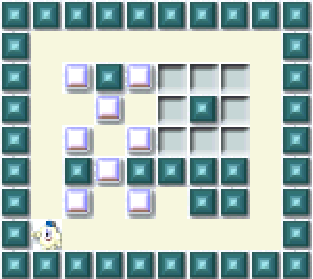
\includegraphics[scale=0.8]{exampleboard.pdf}
\caption*{A typical Sokoban board}
\end{figure}

\section{Approach}
\subsection{Initial idea}
The task was to solve a sokoban board in a maximum of 60 seconds. We
concluded that for boards small boards containing only a few boxes
this should be pretty straight forward. We started out by implementing
a player that just pushed each box in all directions possible, and
saved the resulting states in a stack (a basic DFS search). Of course
this did not work well at all. For the final solution we changed the
search to prioritize moving boxes all the way to a goal area if
possible, and using a priority queue to select which of the saved
states to work on. 

\subsection{The board}
The board is represented internally as a char matrix, and represents the game in one state.
The board contains a list of the positions for all boxes and goals in
the current game state. This later allows us to check the condition of
all boxes in each state quickly. 


Moving a box creates a new game state, and each time we make a move in
one state we copy the old board, instruct it to make a move, and save
the copy. The board representation is thus responsible for checking
that the move made is legal, i.e. the player is not walking on top of
boxes, walls or out of the board.


\subsection{Deadlock detection}
After loading a map into a game state, we try to detect deadlocks. If
we could catch all deadlock situations we could eliminate a lot of the
states that would not work anyways. The problem is that detecting
deadlocks is very difficult, and if done incorrectly could eliminate
states that actually contained the solution we were looking for. We
divided deadlock detection into two groups: Static and Dynamic
deadlocks. 

\subsubsection{Static deadlocks}
Static deadlocks are those that does not change during the game such
as putting a box in a corner with no way to pushing it out of
there. Finding static deadlocks is fairly straightforward and is only
done once for each board, due to their nature of being static. This is
done by simply checking all empty spaces for the following criterion:
if it is a corner or if you can’t pull a box from any of the goals to
the space. This is true because pulling a box is the exact reverse of
pushing it. Thus, if a box can’t be pulled from any goal to a certain
space, then a box can never be pushed to a goal from that space, and
so it is a deadlock.

\subsubsection{Dynamic deadlocks}

Dynamic deadlocks are all sorts of deadlocks that are caused by boxes
blocking each other. A check for these is made whenever a box is
moved, and if a deadlock is detected the state generated by the move
is discarded.

The easiest example of a dynamic deadlock is when a move results in
four box/wall tiles in a square (where at least one of the boxes are
not on a goal):
\begin{table}[h]
\centering
\begin{tabular}{cc}
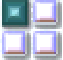
\includegraphics{dd1.pdf} & 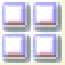
\includegraphics{dd2.pdf}
\end{tabular}
\end{table}

The agent also detects situations where a box is cornered by a wall
and a box, where that box is also cornered by a wall and the
aforementioned box, as in the configurations below:
\begin{table}[h]
\centering
\begin{tabular}{cc}
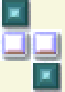
\includegraphics{dd3.pdf} & 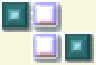
\includegraphics{dd4.pdf}
\end{tabular}
\end{table}

\subsection{Hash table}
It is very inefficient to evaluate the same states multiple times. To
avoid this we implemented a hash function and a Hash table to store
evaluated states in. The hash is, in its default configuration,
calculated as the position of the boxes. It is very simple but unique
for different box positions. A board with two boxes has the same hash
even if the boxes switch positions. We decided to do it like this
because switching positions of two boxes does not help our solution in
anyway.

This hash function, as described above, does not take into account the
position of the player. Doing so would generate a lot of states for
each player position for the same setup of boxes. However, there are
times when player position should be taken into account, such as when
boxes needs to be pushed back and forth through a tunnel. In these
cases the application breaks after some states passed with no
solution. Then we clear the hash table and re-run the application with
the player position in the hash. 

In the cases where we do not need the players position this is a great
performance improvement, and where we do need the player position we
get another try at completing the board.

\subsection{Agent operation}
The agent operates by taking each element in the priority queue,
generate new states from it with different scores (for sorting the
queue), putting these into the queue, and repeating. It generates new
states in two steps: Matching and randomizing.

\subsubsection{Matching}
Matching is done by creating a bipartite graph from all available
(that is, not standing on top of a goal) boxes and all free goals,
using pushable paths between them as edges, and then solving its
maximum matching by reducing it to the maximum flow problem and
solving it with the Edmonds-Karp algorithm. Thus we get a maximum
possible match between free boxes and free goals. The agent takes this
matching, performs the first of the moves in it, and then makes a new
such matching on the resulting board and repeating the process until
no matching is found.

After every move made, the agent saves the resulting state in the
priority queue with a modified score to push it to the front of the
queue (as it is generally a good move).

\subsubsection{Randomizing}
After generating states from the matching process, the state also
generates states by moving the box up, down, left, and right (assuming
it is actually possible to do so) and saving these in the queue. These
have a generally lower score than those generated by the matching, but
are nevertheless necessary in order to explore all options.

\subsubsection{Scoring states}
After a move has been made and a state is generated, the state is run
through deadlock tests, and if it passes these, it is scored by
weighing together distances from all boxes to any goal (closer is
better), how many boxes are on goals, and how many steps were required
to get to it (less is better). The state also inherits its parent’s
score (good moves should generally lead to better moves).

\subsubsection{Looking for good signs}
The last step after generating a state is looking for good situations
generated by the move.
We use two checks, goal pens and no influence push checks.

A goal pen is a goal square surrounded by three wall squares. If a
move results in a box being pushed into such a square, it is awarded a
high score and is, for all succeeding states, treated as a wall square
(since no box can be pushed into it, and it cannot in most
circumstances hinder any other box from reaching a goal).

A ‘no influence’ or ‘tunnel’ push is a push which has no impact on
other boxes, and after which a second push in the same direction can
only be beneficial. Two configurations lead us to draw the conclusion
that a move was a tunnel push:
\begin{table}[h]
\centering
\begin{tabular}{cc}

\includegraphics{good.pdf} & 
\includegraphics{good2.pdf}
\end{tabular}
\end{table}

If a move results in any of these configurations or their rotated
counterparts, we can safely push the box one step further in the same
direction. In this manner, the agent can be said to consider tunnels
as one square.

\subsubsection{End of line}
The agent keeps taking states and generating new ones in this manner
until it finds one with a solved configuration, upon which it returns
the path which it used to get to it as a LRUD string.

\section{Results}
Our matching algorithm combined with ranked random movements proved to
be quite efficient at solving certain kinds of boards, especially
boards with few boxes and few open spaces. This is in part because our
agent quickly discovers which corners and tunnels create deadlock
situations, and because the running time of the matching algorithm and
the number of random movements made for each state depends solely on
the number of boxes on the board. 

On boards requiring a great deal of back and forth movement, our agent
performs very badly, but it really shined in situations where paths to
goals were not obscured by having to make a lot of movements. That is,
if the board was such that a human observer could easily see a
solution, our agent would find it almost immediately, regardless of
how much distance there was to the goal or how many boxes there were. 

The agent is particularly inefficient in open spaces. This is mainly
because there are a lot more possible states in the open space, which
causes the search tree to be much bigger. Because of this, the agent
has problems with most open boards. On the other hand, the agent is
very efficient in tight spaces. For example, it treats long tunnels as
one position on the board. This means that the agent is able to solve
tight boards, that may seem very complex, very efficiently.
\begin{figure}[h]
\centering
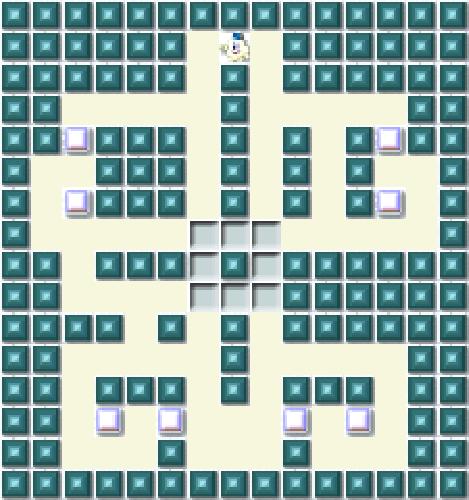
\includegraphics[scale=0.4]{res.pdf}
\caption*{An easy board for our agent}
\end{figure}

\begin{figure}[h]
\centering
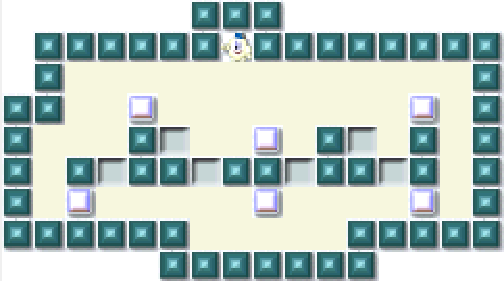
\includegraphics[scale=0.4]{res2.pdf}
\caption*{A hard board for our agent}
\end{figure}
In total, our agent managed to solve 18 out of the 100 test boards,
which must be counted as sub-par performance.
\newpage
\section{Reflection}
When we approached the problem we started out by separating the group
into pairs. Each pair would implement their own agent, then the group
would meet and share ideas and compare the performance of the
agents. The best agent were chosen and developed further. We chose
this approach because it seemed like the best allocation of time in
the beginning of the project, when we didn’t have enough material to
start working on the report. 

This approach failed in some sense, because one of the pairs failed to
implement a working agent. If we could redo the project we would
probably let one pair do most of the coding and one pair do the
report, while having several regular brainstorming sessions with the
whole group.

Our program is the result of using a basic idea about how the search
is to be conducted, analyzing how it behaves in testing, and trying to
find general patterns in behavior considered detrimental to solving
the puzzle. Eliminating static deadlocks, and finding patterns that
give a deadlocked state were generally the easiest challenges, since
they are easily calculated in the beginning of the search and do not
change during the rest of it. The hardest challenge was to determine
and be sure of which moves were beneficial for the agent. 

\end{document}